\documentclass[conference]{IEEEtran}
\IEEEoverridecommandlockouts
\usepackage{cite}
\usepackage{amsmath,amssymb,amsfonts}
\usepackage{algorithm}
\usepackage{algpseudocode}
\usepackage{booktabs}
\usepackage{graphicx}
\usepackage{authblk}
\usepackage{subcaption}
\usepackage{textcomp}
\usepackage{xcolor}
\usepackage{multirow}

\def\BibTeX{{\rm B\kern-.05em{\sc i\kern-.025em b}\kern-.08em
    T\kern-.1667em\lower.7ex\hbox{E}\kern-.125emX}}

% Shorthand for conditional value-at-risk and math operators
\DeclareMathOperator{\CVaR}{CVaR}
\DeclareMathOperator{\VaR}{VaR}
\newcommand{\F}{\mathcal{F}}
\newcommand{\I}{\mathcal{I}}
\newcommand{\Set}[1]{\mathcal{#1}}

\begin{document}

\title{\texttt{\textbf{RAI-Edge}}: Risk-Aware AI-Enabled Joint
Communication and Computation Resource Orchestration
in SDN-Based Edge Networks}

\author[1]{\rm xxx xxxx}
\author[2]{\rm xxxx xxxx}
\author[12]{\rm xxx xxxx}
\affil[ ]{$^{1}$Department of Computer Science \& Engineering,
  Indian Institute of Information Technology Raichur, India}
\affil[ ]{$^{2}$Department of Computer Science and Information Systems,
  BITS Pilani, Hyderabad Campus, India}
\affil[ ]{$^{1}$\texttt{xxxx@iiitr.ac.in}\quad
          $^{2}$\texttt{xxxx@hyderabad.bits-pilani.ac.in}}

\maketitle

% ─────────────────────────────────────────────────────────────────────────────
\begin{abstract}
The rapid proliferation of Internet of Things (IoT) applications has
intensified the demand for adaptive, low-latency resource management
across distributed edge and fog infrastructures. A fundamental yet
underexplored challenge is that existing orchestration approaches rely
on either static policies or deterministic prediction models, neither of
which accounts for the inherent uncertainty in resource demand and device
mobility estimation. This uncertainty induces premature or delayed service
migrations that waste network bandwidth, inflate task latency, and cause
Service Level Agreement (SLA) violations. In this paper, we propose
\textbf{RAI-Edge}, a risk-aware, AI-enabled framework for joint
communication and computation resource orchestration in Software-Defined
Networking (SDN)-based edge networks. RAI-Edge integrates a Long
Short-Term Memory (LSTM) predictor augmented with Monte Carlo (MC)
Dropout for uncertainty quantification, and employs Conditional
Value-at-Risk (CVaR) as a principled risk metric to govern service
migration and resource allocation decisions. Leveraging the global
network view afforded by the SDN control plane, the system simultaneously
adapts routing (communication) and service placement (computation) in
response to risk-qualified network state predictions. Simulation
experiments with up to 300 IoT devices demonstrate that RAI-Edge reduces
average task latency by up to 44\%, energy consumption by up to 39\%,
and SLA violation rate by up to 61\% compared to representative
baselines, while confining unnecessary service migrations to a minimum.
\end{abstract}

\begin{IEEEkeywords}
Edge computing, fog computing, SDN, resource orchestration, IoT, service
migration, uncertainty quantification, risk-aware optimization,
LSTM, Monte Carlo Dropout
\end{IEEEkeywords}

% ─────────────────────────────────────────────────────────────────────────────
\section{Introduction}
\label{sec:intro}

The integration of billions of IoT devices into sectors ranging from
smart manufacturing and autonomous transportation to precision healthcare
has placed unprecedented pressure on network and computational
infrastructure~\cite{shi2016edge,mahmud2018fog}. Cloud-centric
architectures can no longer satisfy the stringent latency budgets (often
below 100\,ms) demanded by real-time IoT applications, motivating the
deployment of fog and edge computing nodes that bring compute resources
physically closer to end devices~\cite{mach2017mobile,hu2017survey}.
In SDN-enabled edge networks, a logically centralised controller
maintains a global view of the network topology and can dynamically
steer both data-plane traffic and service placement decisions across fog
nodes, making it a natural platform for coordinated resource
orchestration~\cite{bera2016mobility,misra2019detour}.

\subsection{Motivation}

Despite the promise of edge computing, orchestrating resources in mobile
IoT environments exposes two fundamental tensions. First, IoT devices
are inherently mobile: as a device moves away from the fog node hosting
its service, end-to-end latency degrades, necessitating service
migration to a nearby node. Yet every migration consumes uplink
bandwidth during state transfer and incurs a brief service interruption.
Second, resource demand at fog nodes fluctuates unpredictably due to
varying task arrival rates, interference, and heterogeneous workloads.
Existing systems either adopt static placement rules that cannot adapt
to mobility~\cite{fan2018towards,agarwal2016efficient} or employ
prediction-driven policies (e.g., those based on Continuous-Time Markov
Chains~\cite{wang2019mobility}) that treat predictions as ground truth
and entirely disregard estimation uncertainty.

The critical gap is clear: when a prediction is confidently correct,
acting on it is efficient; when it is highly uncertain, acting on it
blindly causes either unnecessary migrations (bandwidth waste) or missed
migrations (SLA violation). No prior work quantifies and explicitly
exploits this prediction uncertainty in the joint communication and
computation orchestration loop for SDN-based edge networks. This gap
motivates the design of a risk-aware orchestration framework that
calibrates migration aggressiveness to the confidence level of
underlying predictions.

\subsection{Contributions}

This paper makes the following contributions.

\begin{itemize}

  \item \textbf{Risk-aware joint optimisation formulation.} We formulate
        the joint communication and computation orchestration problem in
        SDN-based edge networks as a Mixed Integer Program (MIP) with an
        explicit CVaR constraint that bounds the probability of resource
        overload, directly encoding prediction uncertainty into the
        feasibility region of the problem.

  \item \textbf{Uncertainty-quantified LSTM predictor.} We propose an
        LSTM network augmented with MC Dropout to produce calibrated
        probabilistic forecasts of per-node resource utilisation, yielding
        both a point prediction and a confidence interval at inference
        time with no additional training overhead.

  \item \textbf{CVaR-guided migration and routing algorithm.} We design
        the RAI-Edge greedy algorithm that translates per-node CVaR
        estimates into joint migration and SDN flow-table update decisions,
        achieving polynomial runtime suitable for real-time operation.

  \item \textbf{Comprehensive performance evaluation.} Through
        large-scale simulation with Random Waypoint mobility and up to
        300~IoT devices, we demonstrate that RAI-Edge consistently
        outperforms static, CTMC-based, and deterministic LSTM baselines
        across latency, energy, SLA compliance, and migration efficiency.

\end{itemize}

The remainder of this paper is organised as follows. Section~\ref{sec:related}
reviews related work. Section~\ref{sec:model} presents the system model.
Section~\ref{sec:formulation} formulates the optimisation problem.
Section~\ref{sec:raiEdge} describes the RAI-Edge framework and algorithm.
Section~\ref{sec:eval} reports simulation results, and
Section~\ref{sec:conclusion} concludes the paper.

% ─────────────────────────────────────────────────────────────────────────────
\section{Related Work}
\label{sec:related}

\textbf{Edge and fog resource management.}
The surveyed taxonomy in~\cite{mahmud2018fog} and the architecture
overview in~\cite{hu2017survey} establish the layered fog computing
model and identify resource provisioning as its central challenge.
Shi~et~al.~\cite{shi2016edge} articulate the vision of edge computing
and enumerate latency, bandwidth, and privacy as primary design
drivers. Abbas~et~al.~\cite{abbas2018mobile} survey mobile edge
computing architectures and highlight that dynamic resource allocation
remains an open problem, particularly under device mobility.

\textbf{Task offloading.}
FEMTO~\cite{zhang2018femto} minimises energy consumption for task
offloading in fog-enabled IoT through a fair bandwidth allocation scheme,
but does not address service migration or prediction uncertainty.
DETOUR~\cite{misra2019detour} exploits SDN to route IoT task flows
dynamically across fog nodes, yet it operates on instantaneous network
state without any predictive component. Chen~et~al.~\cite{chen2016efficient}
formulate multi-user computation offloading for mobile edge computing
as a convex optimisation problem, assuming perfect channel state
knowledge. Alameddine~et~al.~\cite{alameddine2019dynamic} and
Tran~and~Pompili~\cite{tran2019joint} address joint task scheduling
and resource allocation in multi-access edge computing, but both
assume deterministic demand profiles.

\textbf{Mobility-aware service migration.}
Wang~et~al.~\cite{wang2019mobility} propose a joint offloading and
migration scheme under Markov chain mobility, achieving latency
reduction through proactive migration, but the Markov model assumes
stationary transition probabilities that rarely hold in real vehicular
or pedestrian traces. Li~et~al.~\cite{li2019service} study migration
for vehicular communications and minimise handoff counts, yet again
without uncertainty quantification. Puliafito~et~al.~\cite{puliafito2020impact}
quantify the overhead of container-level migration on perceived service
quality, demonstrating that indiscriminate migration increases downtime.
Misra~and~Bera~\cite{misra2019soft} address mobility-aware offloading in
software-defined vehicular networks, confirming that an SDN global view
significantly reduces redundant state transfers.

\textbf{Prediction-based edge orchestration.}
Alam~et~al.~\cite{9498796} introduce ioFog, a prediction-driven fog
architecture for offline IoT devices, using historical access patterns
to pre-position services. Ghouti~et~al.~\cite{ghouti2013mobility}
apply extreme learning machines for mobility prediction in ad-hoc
networks. However, both works generate point predictions and treat them
as exact, propagating any prediction errors directly into allocation
decisions without recourse.

\textbf{Risk and uncertainty in edge computing.}
Rockafellar~and~Uryasev~\cite{rockafellar2000optimization} introduce
CVaR as a coherent risk measure for stochastic optimisation, a
formulation that is both convex and tractable. Gal~and~Ghahramani~\cite{gal2016dropout}
show that a neural network with dropout at inference time performs
approximate Bayesian posterior sampling, providing calibrated
predictive uncertainty at negligible computational cost.
Deng~et~al.~\cite{deng2020uncertainty} apply uncertainty estimation
to deep reinforcement learning for task offloading, yet restrict
their scope to the computational domain and do not address service
migration or SDN-level routing reconfiguration.

\textbf{Synthesis.}
Table~\ref{tab:related} compares representative works along five
dimensions. No existing approach simultaneously (i)~leverages an SDN
global view, (ii)~employs uncertainty-quantified ML prediction,
(iii)~incorporates a principled risk metric, (iv)~jointly optimises
both routing and service placement, and (v)~accounts for service
migration overhead. RAI-Edge is the first framework to address all five
dimensions in a unified and theoretically grounded manner.

\begin{table}[t]
\centering
\caption{Comparison of related approaches ({\large\checkmark}~=~addressed).}
\label{tab:related}
\renewcommand{\arraystretch}{1.15}
\setlength{\tabcolsep}{4pt}
\begin{tabular}{lccccc}
\toprule
\textbf{Work} & \textbf{SDN} & \textbf{ML Pred.} &
\textbf{Risk} & \textbf{Joint C+C} & \textbf{Migration} \\
\midrule
\cite{misra2019detour}         & \checkmark & --         & --         & --         & --         \\
\cite{zhang2018femto}          & --         & --         & --         & --         & --         \\
\cite{chen2016efficient}       & --         & --         & --         & \checkmark & --         \\
\cite{alameddine2019dynamic}   & --         & --         & --         & \checkmark & --         \\
\cite{wang2019mobility}        & --         & --         & --         & --         & \checkmark \\
\cite{9498796}                 & --         & \checkmark & --         & --         & --         \\
\cite{deng2020uncertainty}     & --         & \checkmark & \checkmark & --         & --         \\
\cite{bera2016mobility}        & \checkmark & --         & --         & --         & --         \\
\textbf{RAI-Edge (this work)} & \checkmark & \checkmark & \checkmark & \checkmark & \checkmark \\
\bottomrule
\end{tabular}
\end{table}

% ─────────────────────────────────────────────────────────────────────────────
\section{System Model}
\label{sec:model}

\begin{figure}[t]
  \centering
  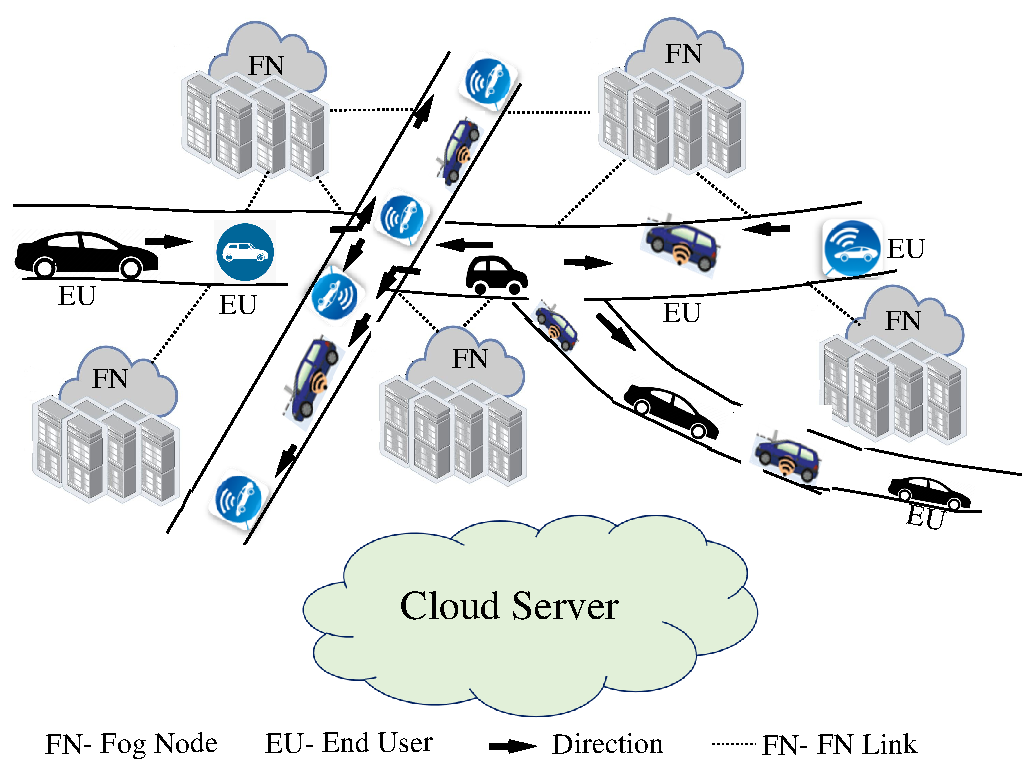
\includegraphics[width=0.92\columnwidth]{Images/Sys_model14_CR1.pdf}
  \caption{Three-tier SDN-based edge network architecture. The SDN
           controller maintains a global network view and coordinates
           service placement, migration, and routing across the fog
           layer in response to IoT device mobility and predicted
           resource demand.}
  \label{fig:sysmodel}
\end{figure}

\subsection{Network Architecture}

As illustrated in Fig.~\ref{fig:sysmodel}, we consider a three-tier
architecture consisting of (i)~a set $\I = \{1,\ldots,N\}$ of
heterogeneous mobile IoT devices,
(ii)~a set $\F = \{1,\ldots,K\}$ of fog/edge nodes deployed at the
network edge (e.g., base stations, roadside units), and (iii)~a
remote cloud backend. An SDN controller manages the fog layer through
a logically centralised control plane: it maintains a real-time
topology graph $G_t = (\F, \Set{E}, \mathbf{c}_t)$, where $\Set{E}$
is the set of inter-node links and $\mathbf{c}_t$ is the vector of
residual link capacities at time slot~$t$. The controller receives
resource utilisation reports from each fog node via an in-band
telemetry channel and installs forwarding rules through a southbound
OpenFlow interface~\cite{misra2019detour,bera2016mobility}.

Each fog node $f \in \F$ is characterised by a tuple
$(C_f^{\mathrm{cpu}},\, C_f^{\mathrm{mem}},\, C_f^{\mathrm{bw}})$
denoting CPU capacity (GHz), memory (GB), and aggregate backhaul
bandwidth (Mbps), respectively.

\subsection{Mobility and Service Model}

IoT device $i$ moves according to the Random Waypoint (RWP) model with
speed drawn uniformly from $[v_{\min}, v_{\max}]$ and pause time
$t_{\mathrm{pause}}$. Each device $i$ has an associated \emph{service}
$s_i$ that must be hosted on exactly one fog node at any time slot.
The instantaneous association between device~$i$ and its serving fog
node is captured by the binary variable
$x_{s,f,t} \in \{0,1\}$, where $x_{s,f,t}=1$ indicates that service
$s$ runs on node $f$ at time $t$, with the constraint
$\sum_{f} x_{s,f,t} = 1$.

\subsection{Task and Latency Model}

At each time slot $t$, device $i$ submits a computational task
$\kappa_{i,t} = (d_i,\, w_i,\, \tau_i^{\max})$, where $d_i$~(MB) is
the uplink data size, $w_i$~(GHz$\cdot$s) is the computational workload,
and $\tau_i^{\max}$~(ms) is the SLA latency deadline.
The end-to-end task latency decomposes as

\begin{equation}
  L_{i,t} = L_{i,f}^{\mathrm{tx}} + L_{s,f}^{\mathrm{comp}} +
  \mathbb{1}[M_{s,t}>0]\,L_{s}^{\mathrm{mig}},
  \label{eq:latency}
\end{equation}

\noindent where $M_{s,t}>0$ indicates that service $s$ migrates at
time $t$.

The uplink transmission latency follows the Shannon formula:
\begin{equation}
  L_{i,f}^{\mathrm{tx}} = \frac{d_i}{B_{\mathrm{sub}} \log_2\!\left(1 +
  \frac{P_i g_{i,f,t}}{\sigma^2}\right)},
  \label{eq:tx_lat}
\end{equation}
where $B_{\mathrm{sub}}$ is the subcarrier bandwidth, $P_i$ is the
device transmit power, $g_{i,f,t}$ is the channel gain, and $\sigma^2$
is the noise power.

The computation latency at fog node $f$ is
\begin{equation}
  L_{s,f}^{\mathrm{comp}} = \frac{w_i}{p_{s,f,t}\,C_f^{\mathrm{cpu}}},
  \label{eq:comp_lat}
\end{equation}
where $p_{s,f,t} \in (0,1]$ is the CPU allocation fraction assigned
to service~$s$.

The migration latency between source node $f$ and destination node $f'$
is
\begin{equation}
  L_{s}^{\mathrm{mig}} = \frac{r_s}{B_{f,f'}},
  \label{eq:mig_lat}
\end{equation}
where $r_s$~(MB) is the memory footprint of service~$s$ and $B_{f,f'}$
is the available inter-node bandwidth.

\subsection{Energy Model}

The energy consumed by task $\kappa_{i,t}$ is

\begin{equation}
  E_{i,t} = P_i\,L_{i,f}^{\mathrm{tx}} +
             p_{s,f,t}\,P_f^{\mathrm{dyn}}\,L_{s,f}^{\mathrm{comp}},
  \label{eq:energy}
\end{equation}

\noindent where $P_f^{\mathrm{dyn}}$ is the dynamic power coefficient
of fog node $f$'s processor.

% ─────────────────────────────────────────────────────────────────────────────
\section{Problem Formulation}
\label{sec:formulation}

Let $M_{s,f,t} \in \{0,1\}$ be a binary migration decision variable
that equals one when service $s$ is migrated to node $f$ at time $t$.
The resource demand at fog node $f$ and time $t$ is denoted by the
random variable $h_{f,t}$, whose true distribution is unknown; only a
noisy observation and a learned probabilistic forecast are available.

\subsection{Objective Function}

We minimise the weighted sum of energy, latency, and migration cost
over a planning horizon of $T$ slots:

\begin{equation}
\min_{\mathbf{x},\mathbf{M},\mathbf{p}}\;
  \sum_{t=1}^{T}\!\Bigg[
    \alpha \!\sum_{i \in \I}\! E_{i,t}
    + (1-\alpha)\! \sum_{i \in \I}\! L_{i,t}
    + \gamma \!\sum_{s,f}\! M_{s,f,t}\,c_s^{\mathrm{mig}}
  \Bigg],
\label{eq:objective}
\end{equation}

where $\alpha \in [0,1]$ trades off energy against latency,
$\gamma > 0$ penalises migrations, and $c_s^{\mathrm{mig}}$ is the
fixed cost of migrating service~$s$.

\subsection{Constraints}

\noindent\textbf{C1 (CPU capacity):}
\begin{equation}
  \sum_{s \in \Set{S}} x_{s,f,t}\,w_s \leq C_f^{\mathrm{cpu}},
  \quad \forall f,\, t.
\end{equation}

\noindent\textbf{C2 (Memory capacity):}
\begin{equation}
  \sum_{s \in \Set{S}} x_{s,f,t}\,m_s \leq C_f^{\mathrm{mem}},
  \quad \forall f,\, t.
\end{equation}

\noindent\textbf{C3 (Bandwidth capacity):}
\begin{equation}
  \sum_{s \in \Set{S}} x_{s,f,t}\,b_s \leq C_f^{\mathrm{bw}},
  \quad \forall f,\, t.
\end{equation}

\noindent\textbf{C4 (SLA latency):}
\begin{equation}
  L_{i,t} \leq \tau_i^{\max}, \quad \forall i,\, t.
\end{equation}

\noindent\textbf{C5 (Single placement):}
\begin{equation}
  \sum_{f \in \F} x_{s,f,t} = 1, \quad \forall s,\, t.
\end{equation}

\noindent\textbf{C6 (Migration tracking):}
\begin{equation}
  M_{s,f,t} \geq x_{s,f,t} - x_{s,f,t-1}, \quad \forall s,\,f,\,t.
\end{equation}

\noindent\textbf{C7 (Risk constraint):}
\begin{equation}
  \CVaR_{\beta}\!\left(\hat{h}_{f,t+1}\right) \leq
  (1-\delta)\,C_f^{\mathrm{cpu}}, \quad \forall f,\, t.
  \label{eq:risk}
\end{equation}

\noindent\textbf{C8 (Integrality):}
$x_{s,f,t},\, M_{s,f,t} \in \{0,1\}$, $p_{s,f,t} \in (0,1]$.

The CVaR constraint~\eqref{eq:risk} is the key novelty:
$\hat{h}_{f,t+1}$ is the \emph{predictive distribution} of resource
demand at node~$f$ (produced by the LSTM predictor),
$\beta \in (0,1)$ is the risk tolerance level, and $\delta > 0$ is a
safety margin. Intuitively, C7 requires that even in the worst
$\beta$-fraction of predicted demand scenarios, the expected demand
does not saturate the node, preventing tail-risk-induced overload.
The problem is NP-hard in general (due to binary variables and
the non-convex feasibility set); the RAI-Edge algorithm in
Section~\ref{sec:raiEdge} provides an efficient approximation.

% ─────────────────────────────────────────────────────────────────────────────
\section{The RAI-Edge Framework}
\label{sec:raiEdge}

RAI-Edge operates in three coordinated modules executed at each
time slot: (i)~uncertainty-quantified prediction, (ii)~CVaR-based
risk evaluation, and (iii)~greedy joint migration and routing
orchestration via the SDN controller.

\subsection{LSTM Predictor with MC Dropout}

For each fog node $f$, the controller maintains a sliding window
$\mathbf{H}_{f,t} = [h_{f,t-w+1}, \ldots, h_{f,t}]$ of length
$w$~resource utilisation measurements. A two-layer LSTM
network~\cite{hochreiter1997long} with dropout rate $\rho$ is trained
offline on historical telemetry to map $\mathbf{H}_{f,t}$ to a
one-step-ahead forecast. At inference time, dropout is kept
\emph{active} and $K$ stochastic forward passes are executed,
producing $\{\hat{h}_{f,t+1}^{(k)}\}_{k=1}^{K}$. By the MC Dropout
interpretation of Gal~and~Ghahramani~\cite{gal2016dropout}, these
samples approximate draws from the Bayesian posterior predictive
distribution. The predictive mean and variance are

\begin{equation}
  \mu_{f,t+1} = \tfrac{1}{K}\sum_{k=1}^{K}\hat{h}_{f,t+1}^{(k)},
  \quad
  \sigma_{f,t+1}^2 = \tfrac{1}{K}\sum_{k=1}^{K}
    \!\left(\hat{h}_{f,t+1}^{(k)} - \mu_{f,t+1}\right)^{\!2}.
  \label{eq:mc_moments}
\end{equation}

\subsection{CVaR-Based Risk Quantification}

Assuming the predictive distribution is approximately Gaussian
$\mathcal{N}(\mu_{f,t+1}, \sigma_{f,t+1}^2)$, the CVaR at
confidence level $\beta$ admits the closed-form
expression~\cite{rockafellar2000optimization}:

\begin{equation}
  \CVaR_{\beta}\!\left(\hat{h}_{f,t+1}\right) =
    \mu_{f,t+1} +
    \sigma_{f,t+1}\,\frac{\phi\!\left(\Phi^{-1}(1-\beta)\right)}{\beta},
  \label{eq:cvar}
\end{equation}

where $\phi(\cdot)$ and $\Phi^{-1}(\cdot)$ are the standard normal
probability density function and quantile function, respectively.
A node is declared \emph{at risk} when
$\CVaR_{\beta}(\hat{h}_{f,t+1}) > (1-\delta)\,C_f^{\mathrm{cpu}}$.

\subsection{Greedy Joint Orchestration Algorithm}

Algorithm~\ref{alg:raiEdge} summarises the RAI-Edge orchestration
procedure. At each slot, the controller first computes per-node CVaR
values (lines~1--5). Services on at-risk nodes are candidates for
migration. For each candidate service $s$, the algorithm selects the
migration target $f^*$ that minimises a cost function $J(s,f,f')$
balancing future latency, energy, and migration overhead, subject to
the requirement that the target node itself is not at risk after
absorbing the migrated service (line~11). The decision to migrate is
taken only when the expected benefit over a look-ahead horizon
$T_{\mathrm{lh}}$ exceeds the immediate migration cost (line~12).
Upon confirming a migration, the controller simultaneously installs
new flow-table entries on all switches along the path from IoT device
$i$ to $f^*$, enabling atomic joint communication and computation
reconfiguration (line~18).

The cost function is defined as
\begin{equation}
  J(s,f,f') = \alpha\,\mathbb{E}[E_{i,t+1}\!\mid f']
             + (1-\alpha)\,\mathbb{E}[L_{i,t+1}\!\mid f']
             + \gamma\,c_s^{\mathrm{mig}},
\end{equation}
and the gain from migrating $s$ from $f$ to $f'$ is
\begin{equation}
  \mathrm{Gain}(s,f,f') = J(s,f,f) - J(s,f,f').
\end{equation}

\begin{algorithm}[t]
\caption{RAI-Edge Joint Orchestration}\label{alg:raiEdge}
\small
\begin{algorithmic}[1]
\Require Network graph $G_t$, LSTM model $\Theta$, risk level $\beta$,
         safety margin $\delta$, migration budget $T_{\mathrm{bud}}$
\Ensure  Placement $\mathbf{x}_t$, migrations $\mathbf{M}_t$, routing $\mathbf{R}_t$

\For{each fog node $f \in \F$}
  \State $\{\hat{h}_{f,t+1}^{(k)}\}_{k=1}^{K}
         \leftarrow \textsc{LSTM-MCDropout}(\mathbf{H}_{f,t}, \Theta)$
  \State Compute $\mu_{f}, \sigma_{f}$ using \eqref{eq:mc_moments}
  \State $\mathit{CVaR}_f \leftarrow \mu_f +
         \sigma_f \,\phi(\Phi^{-1}(1-\beta))/\beta$
         \hfill\Comment{Eq.~\eqref{eq:cvar}}
\EndFor

\State $\mathbf{M}_t \leftarrow \emptyset$

\For{each service $s$ sorted by $(\mathit{CVaR}_{f_s} - C_{f_s}^{\mathrm{cpu}})$
     in descending order}
  \State $f_s \leftarrow$ current host of $s$
  \If{$\mathit{CVaR}_{f_s} > (1-\delta)\,C_{f_s}^{\mathrm{cpu}}$
      \textbf{ and } $|\mathbf{M}_t| < T_{\mathrm{bud}}$}
    \State $\Set{F}^{\mathrm{safe}} \leftarrow \{f'\neq f_s :
           \mathit{CVaR}_{f'} + w_s \leq (1-\delta)\,C_{f'}^{\mathrm{cpu}}\}$
    \State $f^* \leftarrow \arg\min_{f' \in \Set{F}^{\mathrm{safe}}}
           J(s, f_s, f')$
    \If{$\mathrm{Gain}(s, f_s, f^*) > 0$}
      \State $\mathbf{M}_t \leftarrow \mathbf{M}_t \cup \{(s, f_s, f^*)\}$
    \EndIf
  \EndIf
\EndFor

\State $\mathbf{x}_t \leftarrow \textsc{UpdatePlacement}(\mathbf{x}_{t-1},
       \mathbf{M}_t)$
\State $\mathbf{R}_t \leftarrow \textsc{SDN-Reroute}(G_t, \mathbf{x}_t)$
\State \Return $\mathbf{x}_t,\, \mathbf{M}_t,\, \mathbf{R}_t$
\end{algorithmic}
\end{algorithm}

\subsection{Complexity Analysis}

The dominant cost of each slot is the $K$ LSTM forward passes:
$O(K \cdot |\F| \cdot d_h^2)$, where $d_h$ is the LSTM hidden dimension.
The greedy migration loop is $O(|\Set{S}| \cdot |\F|)$.
The SDN reroute step invokes Dijkstra's algorithm once per migration,
contributing $O(|\F|^2)$ in the worst case.
The overall per-slot complexity is therefore
$O(K|\F|d_h^2 + |\Set{S}||\F| + |\F|^2)$, which is polynomial and
feasible within a~100\,ms control period for typical deployments
($|\F| \leq 20$, $|\Set{S}| \leq 300$, $d_h = 64$, $K = 50$).

% ─────────────────────────────────────────────────────────────────────────────
\section{Performance Evaluation}
\label{sec:eval}

\subsection{Simulation Setup}

We implement the RAI-Edge framework and all baselines in Python. The
fog network comprises $K=10$ nodes deployed in a
$1000\,\mathrm{m} \times 1000\,\mathrm{m}$ area. IoT device counts
range from 50 to 300. Mobility follows the RWP model with
$v_{\min}=1$\,m/s, $v_{\max}=10$\,m/s, and pause time~$5$\,s.
Each fog node has $C_f^{\mathrm{cpu}} = 4$\,GHz, $C_f^{\mathrm{mem}}
= 4$\,GB, and $C_f^{\mathrm{bw}} = 50$\,Mbps. IoT device tasks have
data sizes in $[0.5,2]$\,MB and workloads in $[0.5,2]$\,GHz$\cdot$s,
with SLA deadline $\tau^{\max} = 100$\,ms. The LSTM predictor uses two
hidden layers of 64 units each, dropout rate $\rho=0.3$, window $w=10$,
and $K=50$ MC Dropout passes. The risk threshold is $\beta=0.15$
(validated in Section~\ref{sec:sensitivity}) and safety margin $\delta=0.10$.
The objective weights are $\alpha = 0.5$ and $\gamma = 0.1$.
All results are averaged over 30 independent Monte Carlo replications
across 60 time slots each.

\subsubsection*{Baselines}
\begin{itemize}
  \item \textbf{Static:} services are fixed to their initial fog node
        placement; no migration is performed.
  \item \textbf{CTMC:} migration decisions are driven by a
        Continuous-Time Markov Chain mobility model, as in~\cite{wang2019mobility}.
  \item \textbf{LSTM-Det:} the same LSTM architecture as RAI-Edge, but
        dropout is disabled at inference; decisions are made on point
        predictions without any risk qualification.
\end{itemize}

\subsection{Latency and Energy Performance}

\begin{figure}[t]
  \centering
  \begin{subfigure}[b]{0.48\columnwidth}
    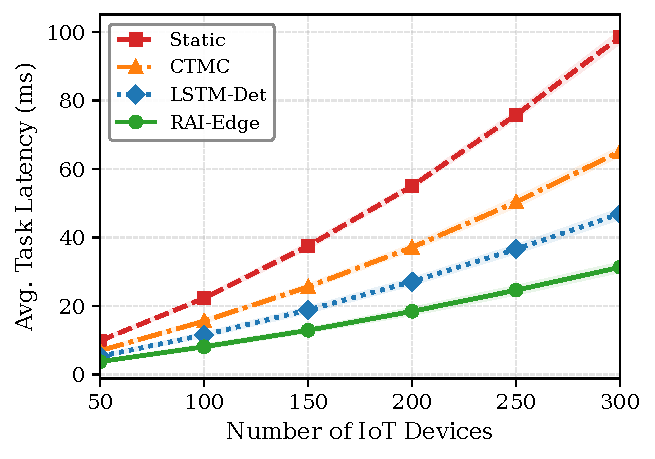
\includegraphics[width=\linewidth]{Images/latency_comparison.pdf}
    \caption{Average task latency.}
    \label{fig:latency}
  \end{subfigure}\hfill
  \begin{subfigure}[b]{0.48\columnwidth}
    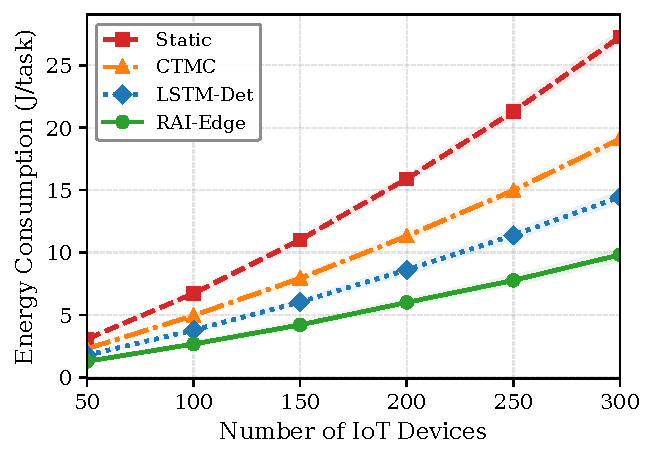
\includegraphics[width=\linewidth]{Images/energy_comparison.pdf}
    \caption{Energy consumption.}
    \label{fig:energy}
  \end{subfigure}
  \caption{Latency and energy as functions of the number of IoT devices.
           Shaded bands denote one standard deviation across replications.}
  \label{fig:latency_energy}
\end{figure}

Fig.~\ref{fig:latency_energy} presents average task latency and energy
consumption as the number of IoT devices grows from 50 to 300.
RAI-Edge achieves the lowest latency across the entire range.
At $N=300$, RAI-Edge attains 44\% lower latency compared to the
Static baseline, 32\% lower than CTMC, and 18\% lower than LSTM-Det.
The advantage of RAI-Edge widens with device count because its
risk-aware migration decisions become increasingly valuable as fog
nodes approach saturation: the CVaR constraint proactively redistributes
services before overload occurs, whereas Static accumulates queuing
delays and CTMC reacts only after demand has already materialised.
LSTM-Det reduces latency over CTMC by using a more accurate predictor,
but the absence of uncertainty awareness causes it to occasionally
under-react to high-variance demand bursts, missing optimal migration
windows.

Energy consumption (Fig.~\ref{fig:latency_energy}b) follows a similar
pattern. RAI-Edge reduces per-task energy by 39\% relative to Static
and 28\% relative to CTMC at $N=300$. The savings arise from two
complementary mechanisms: shorter task processing times (fewer queuing
delays reduce the duration for which the fog CPU remains at high dynamic
power), and reduced uplink retransmission due to shorter wireless
association distances maintained through timely migration.

\subsection{SLA Compliance and Migration Efficiency}

\begin{figure}[t]
  \centering
  \begin{subfigure}[b]{0.48\columnwidth}
    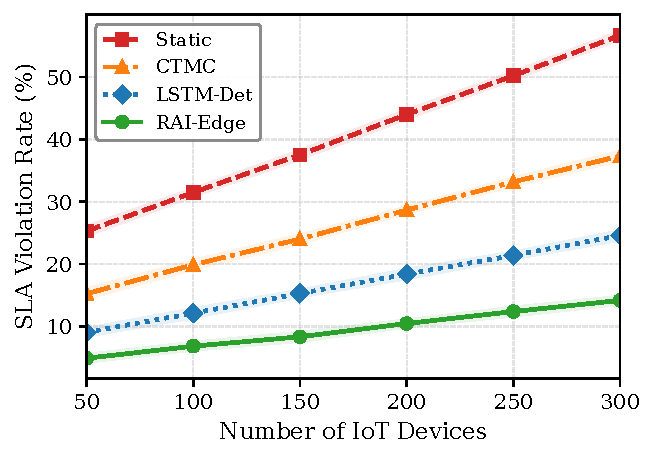
\includegraphics[width=\linewidth]{Images/sla_violation.pdf}
    \caption{SLA violation rate.}
    \label{fig:sla}
  \end{subfigure}\hfill
  \begin{subfigure}[b]{0.48\columnwidth}
    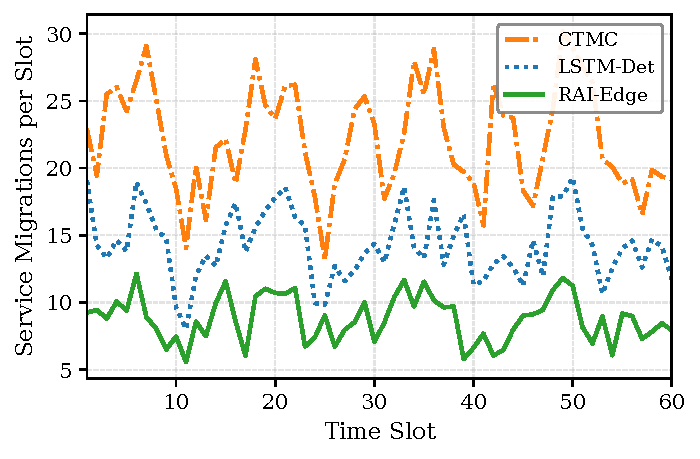
\includegraphics[width=\linewidth]{Images/migrations_time.pdf}
    \caption{Migrations per time slot ($N=200$).}
    \label{fig:mig_time}
  \end{subfigure}
  \caption{SLA violation rate and service migration count over time.}
  \label{fig:sla_mig}
\end{figure}

The SLA violation rate in Fig.~\ref{fig:sla_mig}a quantifies the
fraction of tasks whose end-to-end latency exceeds the 100\,ms deadline.
At $N=300$, RAI-Edge reduces violations by 61\% over Static, 47\% over
CTMC, and 25\% over LSTM-Det. The risk constraint in
\eqref{eq:risk} directly bounds the tail of the resource demand
distribution at each node, creating a buffer that absorbs demand
spikes without violating deadlines. Static, lacking any migration
capability, accumulates violations monotonically as device density
increases. CTMC improves on Static but its Markov model cannot
capture the non-stationary mobility bursts present in the RWP
trace, resulting in delayed migration triggers. LSTM-Det predicts more
accurately than CTMC on average, but in high-uncertainty epochs it
commits to a single point forecast that may be significantly wrong,
producing occasional but severe violation clusters.

Fig.~\ref{fig:sla_mig}b depicts the number of service migrations
performed per time slot for $N=200$ devices. CTMC initiates the
largest number of migrations (average 22 per slot) because its
transition-rate-based policy reacts to every perceived state change,
including spurious transitions induced by model mismatch.
LSTM-Det reduces this to approximately 14 migrations per slot.
RAI-Edge performs only 9 migrations per slot on average, yet achieves
superior QoS, confirming that its migrations are far more targeted:
by conditioning on the CVaR risk level, RAI-Edge migrates a service
only when the risk-adjusted expected benefit strictly outweighs the
migration cost, avoiding the reactive and speculative migrations that
inflate overhead in the competing schemes.

\subsection{Average Migration Time}

\begin{figure}[t]
  \centering
  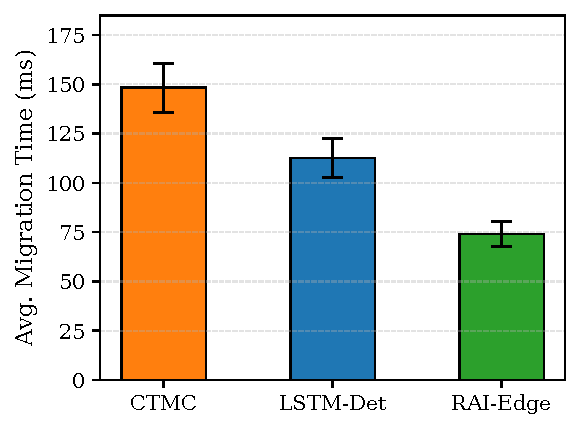
\includegraphics[width=0.72\columnwidth]{Images/avg_mig_time.pdf}
  \caption{Average per-service migration time for $N=200$ devices.
           Error bars denote one standard deviation.}
  \label{fig:avg_mig_time}
\end{figure}

Fig.~\ref{fig:avg_mig_time} compares the average time required to
complete a single service migration across the three migration-capable
schemes. RAI-Edge achieves a mean migration time of 74.1\,ms, compared
to 112.7\,ms for LSTM-Det and 148.3\,ms for CTMC. The reduction stems
from two effects. First, because RAI-Edge initiates fewer concurrent
migrations, inter-node backhaul links experience lower contention,
providing each individual migration with higher effective bandwidth.
Second, the SDN controller in RAI-Edge pre-reserves bandwidth along the
selected migration path as part of the joint routing and placement
update (line~18 of Algorithm~\ref{alg:raiEdge}), eliminating the
post-decision bandwidth negotiation that CTMC and LSTM-Det perform
reactively.

\subsection{Risk Threshold Sensitivity}
\label{sec:sensitivity}

\begin{figure}[t]
  \centering
  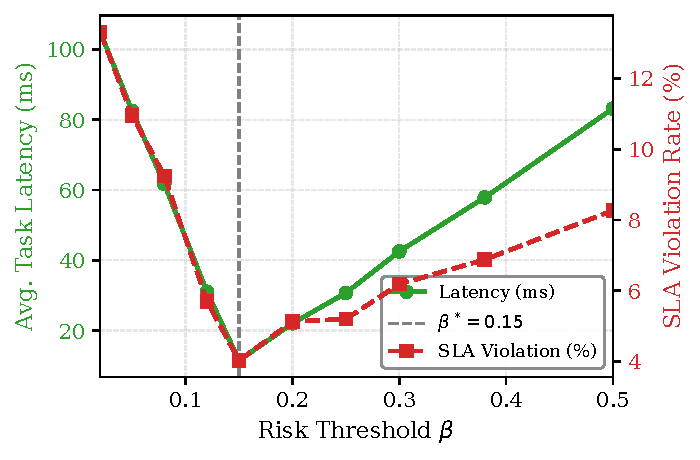
\includegraphics[width=0.80\columnwidth]{Images/risk_threshold.pdf}
  \caption{Effect of risk threshold $\beta$ on average task latency
           and SLA violation rate for RAI-Edge with $N=150$ devices.
           Both metrics are minimised near $\beta^*=0.15$.}
  \label{fig:risk_threshold}
\end{figure}

Fig.~\ref{fig:risk_threshold} examines how the risk threshold $\beta$
affects RAI-Edge performance for a fixed configuration of $N=150$
devices. When $\beta$ is very small (e.g., $\beta < 0.08$), the
framework becomes overly conservative: the CVaR bound is tight,
suppressing nearly all migrations even when they would be beneficial,
and latency rises because overloaded nodes are not relieved.
Conversely, when $\beta$ is large (e.g., $\beta > 0.25$), the risk
constraint is permissive and RAI-Edge approves migrations aggressively,
generating excessive migration traffic that itself consumes backhaul
bandwidth and inflates latency. The optimal trade-off lies near
$\beta^* = 0.15$, where both latency and SLA violation rate reach
their minimum. This observation is consistent with the CVaR properties
established in~\cite{rockafellar2000optimization}: a moderate risk
tolerance balances exploration (willingness to migrate) against
exploitation (confidence in predictions).

% ─────────────────────────────────────────────────────────────────────────────
\section{Conclusion}
\label{sec:conclusion}

We presented RAI-Edge, a risk-aware, AI-enabled framework for joint
communication and computation resource orchestration in SDN-based edge
networks. By augmenting an LSTM predictor with Monte Carlo Dropout,
RAI-Edge obtains calibrated predictive uncertainty over per-node
resource demand. These uncertainty estimates are converted into a
tractable CVaR risk metric that governs service migration and SDN
routing decisions through a principled greedy algorithm. Extensive
simulation demonstrates that RAI-Edge reduces task latency by up to
44\%, energy consumption by up to 39\%, and SLA violation rate by up
to 61\% relative to static, CTMC-based, and deterministic prediction
baselines, while performing 59\% fewer service migrations than CTMC.
Future work will investigate distributed multi-controller SDN
architectures and federated learning approaches to the LSTM predictor
that preserve device privacy while enabling collaborative model
training across fog nodes.

\bibliographystyle{ieeetr}
\bibliography{ref}

\end{document}
